\documentclass{CUP-JNL-DCE}


%%%% Packages
\usepackage{latexsym}
\usepackage{graphicx}
\usepackage{multicol,multirow}
\usepackage{amsmath,amssymb,amsfonts}
\usepackage{mathrsfs}
\usepackage{amsthm}
\usepackage{apacite}
\usepackage{rotating}
\usepackage{appendix}
\usepackage[authoryear]{natbib}
%%%%

\articletype{RESEARCH ARTICLE}
\jname{Data-Centric Engineering}
%\artid{20}
\jyear{2020}
%\jvol{4}
%\jissue{1}
%\doi{2190-8567}
%\raggedbottom

\DeclareGraphicsRule{.tif}{eps}{.tif.bb}{`tiff2ps #1}

\begin{document}

\begin{Frontmatter}

\title[Constructing Digital Twins for Manufacturing]
{Hidden Markov Model based Digital Twin Construction for Futuristic Manufacturing Systems}

\author[1]{Angkush Kumar Ghosh}
\author*[2]{AMM Sharif Ullah}\email{ullah@mail.kitami-it.ac.jp}
\author[2]{Akihiko Kubo}

\authormark{Angkush Kumar Ghosh \textit{et al.}}

\address[1]{\orgdiv{Graduate School of Engineering}, \orgname{Kitami Institute of Technology}, \orgaddress{\street{165 Koen-cho}, \state{Kitami}, \postcode{Hokkaido 090-8507}, \country{Japan}}}

\address*[2]{\orgdiv{Faculty of Engineering}, \orgname{Kitami Institute of Technology}, \orgaddress{\street{165 Koen-cho}, \state{Kitami}, \postcode{Hokkaido 090-8507}, \country{Japan}}}

%$^{\# }$Corresponding Author Tel/Fax: +81-157-26-9207

\keywords{Hidden Markov Model; Digital Twin; Complex Phenomena;
Manufacturing Systems; Surface Roughness}

\abstract{Abstracts should be 250 words. It must be able to stand alone and so cannot contain citations to the paper's references, equations, etc. An abstract must consist of a single paragraph and be concise. Because of online formatting, abstracts must appear as plain as possible. }

\begin{policy}[Impact Statement]
Provide a 200 word impact statement that summarises the significance of the work, so that it can be quickly grasped by a wide audience (including industry, government and wider academia).
\end{policy}

\end{Frontmatter}


\section{Introduction}
\label{sec1}

The aerospace community has introduced a system engineering concept called
digital twin, which refers to an exact mirror image of a real-life aspect
(e.g., flying of a spacecraft) in the cyberspace using the multi-scale,
multi-physics, and probabilistic simulation that is aided by the sensor
updates and historical data (Glaessgen and Stargel 2012). This has inspired
the research community of the futuristic manufacturing systems (e.g.,
Industry 4.0, smart manufacturing, and connected factory). As such, the
digital twins of manufacturing aspects are expected to populate the systems
(e.g., cyber-physical systems) that are needed for functionalizing the
futuristic manufacturing systems (Grieves and Vickers 2017; \citealt{Ullah2019}).
The research on digital twin construction reports its myriad interplays with
various aspects of futuristic manufacturing systems. Some of the recent
articles are described below.

Nevertheless, from the viewpoint of contents, the digital twins can be
categorized into three categories, namely, object twin, process twin, and
phenomenon twin \citep{Ullah2019}. An object twin is the computable virtual
abstraction of the geometrical and topological structures of a product
(e.g., a gear) or a facility (a machine tool, an assembly line, and so
forth). A process twin is a computable virtual abstraction of a process or
production plan (e.g., scheduling for machining a part at different
workstations spread in different factories, a bill of materials, and so
forth). On the other hand, the computable virtual abstraction of a
manufacturing phenomenon (e.g., the phenomena related to material removal
process, namely, cutting force, tool wear, cutting temperature, workpiece
deformation, surface roughness, chatter vibration, and so forth) is called a
phenomenon twin. The three categories of digital twins must populate the
systems (e.g., cyber-physical systems) underlying futuristic manufacturing
systems, as mentioned above.

Section~\ref{sec2} is organized in three subsections to describe the methodology
showing how to construct a hidden Markov model for an arbitrary time series.
Section~\ref{sec3} describes a case study where the methodology described in
Section~\ref{sec2} is applied to create the digital twins of the surface roughness of ground
surface (i.e., the workpiece surface generated by successive grinding
operations).

\section{Methodology}
\label{sec2}

This section describes a methodology showing how to construct a hidden
Markov model using the information of an arbitrary time series. For the sake
of better understanding, this section first describes the fundamental idea,
which is followed by the mathematical formulations and algorithms,
respectively.


\subsection{Fundamental Idea}
\label{sec2.1}

The fundamental idea means here a somewhat informal description of the
hidden Markov model and its relationship with a time series.


\section{Data and Numerical Models}
\label{sec3}

The computing power of hidden Markov models has been playing an important
role in studying the complex phenomena underlying design and manufacturing.
For example, \cite{Liao2016} have\break developed a heuristic optimization
algorithm using hidden Markov model coupled with simulated annealing for
condition monitoring of machineries. \cite{Li2018} have developed a
data-driven bearing fault identification methodology using an improved
hidden Markov model and self-organizing map. \cite{Mba2018} developed a
hidden Markov model based methodology for condition monitoring of gearbox.
\cite{Zhang2018} developed a methodology for predicting the residual life
of the rolling machine elements using hidden Markov model. \cite{Xie2016}
described the hidden Markov model based methodology for recognizing the
machining states ensuring the safe operations. \cite{Bhat2016} developed
a hidden Markov model based tool condition monitoring methodology ensuring
the economical usages of cutting tools. \cite{Liao2006} developed a
grinding wheel condition monitoring methodology where a hidden Markov model
based clustering approach was used to recognize the patterns found in the
acoustic emission signals. \cite{Cai2018} developed a methodology using
hidden Markov model to identify the energy efficiency states while removing
materials by milling ensuring eco-friendly machining operation. \cite{Kumar2018}
integrated hidden Markov model with polynomial regression for
predicting the useful life of cutting tools. Nevertheless, this case study
shows how to apply the hidden Markov model (presented in Section~\ref{sec2}) for
constructing a phenomenon twin of surface roughness. The description is as
follows.

Grinding is a widely used material removal process that helps remove
materials from the surfaces of the objects made of difficult-to-cut
materials (e.g., stainless steels, ceramics, and so forth) ensuring a high
surface finish. In grinding, a complex microscopic interaction between the
abrasive grains attached on the circumferential surface of grinding wheel
and work-surface takes place \citep{Ullah2019}.


\section{Equations}

Equations in \LaTeX{} can either be inline or on-a-line by itself. For
inline equations use the \verb+$...$+ commands. Eg: The equation
$H\psi = E \psi$ is written via the command $H \psi = E \psi$.

For on-a-line by itself equations (with auto generated equation numbers)
one can use the equation or eqnarray environments \textit{D}.
\begin{equation}
\mathcal{L} = i {\psi} \gamma^\mu D_\mu \psi
    - \frac{1}{4} F_{\mu\nu}^a F^{a\mu\nu} - m {\psi} \psi
\label{eq1}
\end{equation}
where,
\begin{align}
D_\mu &=  \partial_\mu - ig \frac{\lambda^a}{2} A^a_\mu
\nonumber \\
F^a_{\mu\nu} &= \partial_\mu A^a_\nu - \partial_\nu A^a_\mu
    + g f^{abc} A^b_\mu A^a_\nu
\label{eq2}
\end{align}
Notice the use of \verb+\nonumber+ in the align environment at the end
of each line, except the last, so as not to produce equation numbers on
lines where no equation numbers are required. The \verb+\label{}+ command
should only be used at the last line of an align environment where
\verb+\nonumber+ is not used.
\begin{equation}
Y_\infty = \left( \frac{m}{\textrm{GeV}} \right)^{-3}
    \left[ 1 + \frac{3 \ln(m/\textrm{GeV})}{15}
    + \frac{\ln(c_2/5)}{15} \right]
\end{equation}
The class file also supports the use of \verb+\mathbb{}+, \verb+\mathscr{}+ and
\verb+\mathcal{}+ commands. As such \verb+\mathbb{R}+, \verb+\mathscr{R}+
and \verb+\mathcal{R}+ produces $\mathbb{R}$, $\mathscr{R}$ and $\mathcal{R}$
respectively.


\section{Figures}

As per the \LaTeX\ standards eps images in \verb!latex! and pdf/jpg/png images in
\verb!pdflatex! should be used. This is one of the major differences between \verb!latex!
and \verb!pdflatex!. The images should be single page documents. The command for inserting images
for latex and pdflatex can be generalized. The package that should be used
is the graphicx package. See Figure \ref{fig1}.

\begin{figure}[!h]%figure 1
\FIG{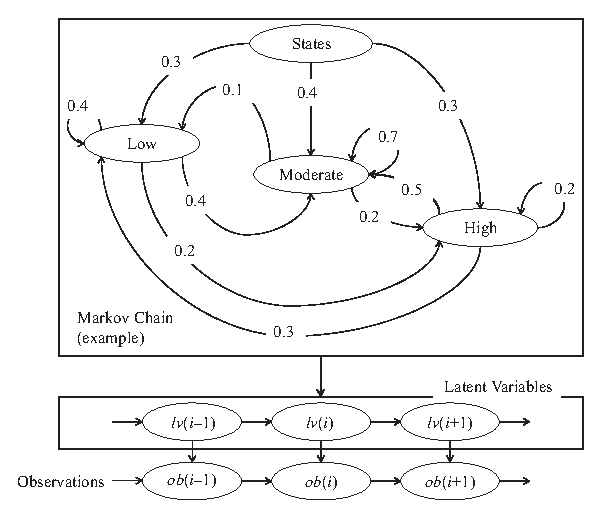
\includegraphics{Figure1.eps}}
{\caption{The concept of hidden Markov model}\label{fig1}}
\vspace*{-22pt}
\end{figure}


\section{Tables}

Tables can be inserted via the normal table and tabular environment. To put
footnotes inside tables one has to use the additional ``fntable" environment
enclosing the tabular environment. The footnote appears just below the table
itself. See Table \ref{tab2}.

%\begin{table}[h]
%\TBL{\caption{Caption text.\label{tab1}}}
%{%
%\begin{tabular}{@{}llll@{}}\toprule
%\TCH{column 1} & \TCH{column 2}  & \TCH{column 3} &
%\TCH{column 4}\\\midrule
%row 1    & data 1   & data 2  & data 3  \\
%row 2    & data 4   & data 5  & data 6  \\
%row 3    & data 7   & data 8  & data 9  \\\botrule
%\end{tabular}}
%\end{table}
%%

\begin{table}[!t]
\tabcolsep=0pt%
\TBL{\caption{Tables which are too long to fit,
should be written using the ``table*" environment as shown here\label{tab2}}}
{\begin{fntable}
\begin{tabular*}{\textwidth}{@{\extracolsep{\fill}}lcccccc@{}}\toprule%
 & \multicolumn{3}{@{}c@{}}{\TCH{Element 1}}& \multicolumn{3}{@{}c@{}}{\TCH{Element 2\smash{\footnotemark[1]}}}
 \\\cmidrule{2-4}\cmidrule{5-7}%
\TCH{Projectile} & \TCH{Energy} & \TCH{$\sigma_{\mathit{calc}}$} & \TCH{$\sigma_{\mathit{expt}}$} &
\TCH{Energy} & \TCH{$\sigma_{\mathit{calc}}$} & \TCH{$\sigma_{\mathit{expt}}$} \\\midrule
\TCH{Element 3}&990 A &1168 &$1547\pm12$ &780 A &1166 &$1239\pm100$\\
{\TCH{Element 4}}&500 A &961 &$922\pm10$ &900 A &1268 &$1092\pm40$\\
\botrule
\end{tabular*}%
\footnotetext{\textbf{Note:} This is an example of table footnote this is an example of table footnote this is an example of table footnote this is an example of~table footnote this is an example of table footnote}
\footnotetext[1]{This is an example of table footnote}%
\end{fntable}}
\end{table}









\section{Cross referencing}

Environments such as figure, table, equation, align can have a label
declared via the \verb+\label{#label}+ command. For figures and table
environments one should use the \verb+\label{}+ command inside or just
below the \verb+\caption{}+ command.  One can then use the
\verb+\ref{#label}+ command to cross-reference them. As an example, consider
the label declared for Figure \ref{fig1} which is
\verb+\label{fig1}+. To cross-reference it, use the command
\verb+ Figure \ref{fig1}+, for which it comes up as
``Figure \ref{fig1}".
The reference citations should used as per the "natbib" packages. Some sample citations:  \cite{Alam2017,Chui2013,Oliveira2017,Talkhestani2018}.


\vspace*{-5pt}
\section{Lists}

List in \LaTeX{} can be of three types: enumerate, itemize and description.
In each environments, new entry is added via the \verb+\item+ command.
Enumerate creates numbered lists, itemize creates bulleted lists and
description creates description lists.
List in \LaTeX{} can be of three types: enumerate, itemize and description.
In each environments, new entry is added via the \verb+\item+ command.
Enumerate creates numbered lists, itemize creates bulleted lists and
description creates description lists.
\begin{enumerate}[1.]
\item This is the 1st item
\item Enumerate creates numbered lists, itemize creates bulleted lists and
description creates description lists.
\item Numbered lists continue.
\end{enumerate}
List in \LaTeX{} can be of three types: enumerate, itemize and description.
In each environments, new entry is added via the \verb+\item+ command.
\begin{itemize}
\item This is the 1st item
\item Itemize creates bulleted lists and
description creates description lists.
\item Bullet lists continue.
\end{itemize}

\vspace*{-12pt}
\section{Conclusion}

Some Conclusions here.


\begin{Backmatter}

\paragraph{Acknowledgments}
We are grateful for the technical assistance of A. Author.


\paragraph{Funding statement}
This research was supported by grants from the <funder-name><doi>(<award ID>); <funder-name><doi>(<award ID>).

\paragraph{Competing interests}
A statement about any financial, professional, contractual or personal relationships or situations that could be perceived to impact the presentation of the work --- or `None' if none exist

\paragraph{Data availability statement}
A statement about how to access data, code and other materials allowing users to understand, verify and replicate findings --- e.g. Replication data and code can be found in Harvard Dataverse: \verb+\url{https://doi.org/link}+.

\paragraph{Ethical standards}
The research meets all ethical guidelines, including adherence to the legal requirements of the study country.

\paragraph{Author contributions}
Please provide an author contributions statement using the CRediT taxonomy roles as a guide {\verb+\url{https://www.casrai.org/credit.html}+}. Conceptualization: A.A; A.B. Methodology: A.A; A.B. Data curation: A.C. Data visualisation: A.C. Writing original draft: A.A; A.B. All authors approved the final submitted draft.

\paragraph{Supplementary material}
State whether any supplementary material intended for publication has been provided with the submission.

\bibliographystyle{apalike}
%\bibliography{Sample-refs}

\begin{thebibliography}{}

\bibitem[Alam and Saddik(2017)]{Alam2017}
Alam, K. M. {\&} Saddik, A. E. (2017). C2PS: A Digital Twin Architecture
Reference Model for the Cloud-Based Cyber-Physical Systems. \textit{IEEE Access}, 5:2050--2062.

\bibitem[Bhat et~al.(2016)]{Bhat2016}
Bhat, N. N., Dutta, S., Pal, S. K., {\&} Pal, S. (2016). Tool condition
classification in turning process using hidden Markov model based on texture
analysis of machined surface images. \textit{Measurement}, 90:500--509.

\bibitem[Cai et~al.(2018)]{Cai2018}
Cai, Y., Shi, X., Shao, H., Wang, R., {\&} Liao, S. (2018). Energy
efficiency state identification in milling processes based on information
reasoning and Hidden Markov Model. \textit{Journal of Cleaner Production}, 193:397--413.

\bibitem[Chui et~al.(2013)]{Chui2013}
Chui, M. W., Feng, Y. Q., Wang, W., Li, P. L., {\&} Li, Z. C. (2013).
Numerical Simulation of Rough Surface with Crossed Texture. \textit{Applied Mechanics and Materials, 321--324}, 196--200.

\bibitem[Fill(2017)]{Fill2017}
Fill, H.-G. (2017). SeMFIS: A flexible engineering platform for semantic
annotations of conceptual models. \textit{Semantic Web}, 8(5):747--763.

\bibitem[Fraser(2008)]{Fraser2008}
Fraser, A. M. (2008). \textit{Hidden Markov models and dynamical systems}. Philadelphia: SIAM.

\bibitem[Kumar et~al.(2018)]{Kumar2018}
Kumar, A., Chinnam, R.B., {\&} Tseng, F. (2018). An HMM and polynomial
regression based approach for remaining useful life and health state
estimation of cutting tools. \textit{Computers {\&} Industrial Engineering}, 128:1008--1014.


\bibitem[Li et~al.(2018)]{Li2018}
Li, Z., Fang, H., Huang, M., Wei, Y., {\&} Zhang, L. (2018). Data-driven
bearing fault identification using improved hidden Markov model and
self-organizing map. \textit{Computers {\&} Industrial Engineering}, 116:37--46.

\bibitem[Liao et~al.(2006)]{Liao2006}
Liao, T. W., Hua, G., Qu, J., {\&} Blau, P. J. (2006). Grinding Wheel
Condition Monitoring with Hidden Markov Model-based Clustering Methods.
\textit{Machining Science {\&} Technology: An International Journal}, 10(4):511--538.

\bibitem[Liao et~al.(2016)]{Liao2016}
Liao, W., Li, D., {\&} Cui, S. (2016). A heuristic optimization algorithm
for HMM based on SA and EM in machinery diagnosis. \textit{Journal of Intelligent Manufacturing}, 29(8):1845--1857.

\bibitem[Mba et~al.(2018)]{Mba2018}
Mba, C. U., Makis, V., Marchesiello, S., Fasana, A., {\&} Garibaldi, L.
(2018). Condition monitoring and state classification of gearboxes using
stochastic resonance and hidden Markov models. \textit{Measurement}, 126:76--95.

\bibitem[Nguyen(2017)]{Nguyen2017}
Nguyen, N. (2017). An Analysis and Implementation of the Hidden Markov Model
to Technology Stock Prediction. \textit{Risks}, 5(4):62:1--62:18.

\bibitem[Oliveira et~al.(2017)]{Oliveira2017}
Oliveira, W., Ambr\'{o}sio, L. M., Braga, R., Str\"{o}ele, V., David, J. M.,
{\&} Campos, F. (2017). A Framework for Provenance Analysis and
Visualization. \textit{Procedia Computer Science}, 108:1592--1601.

\bibitem[Padovano et~al.(2018)]{Padovano2018}
Padovano, A., Longo, F., Nicoletti, L., {\&} Mirabelli, G. (2018). A Digital
Twin based Service Oriented Application for a 4.0 Knowledge Navigation in
the Smart Factory. \textit{IFAC-PapersOnLine}, 51(11):631--636.

\bibitem[Qi et~al.(2018)]{Qi2018}
Qi, Q., Tao, F., Zuo, Y., {\&} Zhao, D. (2018). Digital Twin Service towards
Smart Manufacturing. \textit{Procedia CIRP}, 72:237--242.

\bibitem[Ramos(2015)]{Ramos2015}
Ramos, L. (2015). Semantic Web for manufacturing, trends and open issues:
Toward a state of the art. \textit{Computers {\&} Industrial Engineering}, 90:444--460.

\bibitem[Talkhestani et~al.(2018)]{Talkhestani2018}
Talkhestani, B. A., Jazdi, N., Schloegl, W., {\&} Weyrich, M. (2018).
Consistency check to synchronize the Digital Twin of manufacturing
automation based on anchor points. \textit{Procedia CIRP}, 72:159--164.

\bibitem[Ullah(2019)]{Ullah2019}
Ullah, AMM S. (2019). Modeling and simulation of complex manufacturing
phenomena using sensor signals from the perspective of Industry 4.0.
\textit{Advanced Engineering Informatics}, 39(1):1--13.

\bibitem[Ullah(2017)]{Ullah2017}
Ullah, A. M. M. S. (2017). Surface Roughness Modeling Using Q-Sequence.
\textit{Mathematical and Computational Applications}, 22(2):33:1--33:12

\bibitem[Visser(2011)]{Visser2011}
Visser, I. (2011). Seven things to remember about hidden Markov models: A
tutorial on Markovian models for time series. \textit{Journal of Mathematical Psychology}, 55(6):403--415.

\bibitem[Wu et~al.(2016)]{Wu2016}
Wu, D., Terpenny, J., {\&} Schaefer, D. (2016). Digital design and
manufacturing on the cloud: A review of software and services. \textit{Artificial Intelligence for Engineering Design, Analysis and Manufacturing}, 31(1):104--118.

\bibitem[Xie et~al.(2016)]{Xie2016}
Xie, F.-Y., Hu, Y.-M., Wu, B., {\&} Wang, Y. (2016). A generalized hidden
Markov model and its applications in recognition of cutting states.
\textit{International Journal of Precision Engineering and Manufacturing}, 17(11):1471--1482.

\bibitem[Zhang et~al.(2018)]{Zhang2018}
Zhang, S., Zhang, Y., {\&} Zhu, J. (2018). Residual life prediction based on
dynamic weighted Markov model and particle filtering. \textit{Journal of Intelligent Manufacturing}, 29(4):753--761.

\end{thebibliography}


\end{Backmatter}

\end{document}
